\documentclass[12pt]{beamer}

    \usepackage[spanish, es-tabla]{babel}
    \selectlanguage{spanish}
    \usepackage[utf8]{inputenc}
    \usepackage{listings, xcolor}
    \usepackage{graphicx}

    \graphicspath{ {images/} }
    
    \lstset{
        basicstyle={\small\ttfamily},
        numbers=none,
        breaklines=true,
        breakatwhitespace=true,
        string=[s]{"}{"},
        stringstyle=\color{blue},
        comment=[l]{:},
        commentstyle=\color{black}
    }

    \usetheme{Madrid}
    \AtBeginSection[]
    {
        \begin{frame}
            \frametitle{Índice}
            \tableofcontents[currentsection]
        \end{frame}
    }

    \begin{document}

        \title[Pipeline Análisis IoT]{
            Pipeline para el Análisis en  \\
            Tiempo Real de datos IoT }
        \subtitle{Trabajo de Investigación}
        
        \institute[]{
            Internet de las Cosas en el Contexto de Big Data \\
            Máster en Tecnologías de Análisis de Datos Masivos: Big Data
        }

        \author{Adrián Miralles Palazón}
        \date{\today}
        \logo{
\includegraphics[height=1.5cm]{logo}}

        \maketitle

        \begin{frame}
            \frametitle{Índice}
            \tableofcontents
        \end{frame}

        \section{Introducción}

        \begin{frame}
            \frametitle{Introducción}

            \begin{itemize}
                \item Crecimiento y madurez de ecosistema IoT
                \item Proliferación de tecnologías y herramientas para resolver las distintas tareas a las que se enfrentan los que trabajan con datos
            \end{itemize}
        \end{frame}

        \section{Motivación y Objetivos}

        \begin{frame}
            \frametitle{Motivación y Objetivos}

            \textbf{Motivación} 
            \begin{itemize}
                \item Nula opción a hacer proyectos distintos en el Máster
                \item Es difícil tener tiempo para probar nuevas tecnologías
                \item Construir proyecto desde cero
            \end{itemize}

            \textbf{Objetivos}
            \begin{itemize}
                \item Crear un \textit{data pipeline} desde cero
                \item Todas las tecnologías que se usen, deben ser distintas a las vistas en el Máster
            \end{itemize}
        \end{frame}

        \section{Estado de arte}

        \begin{frame}
            \frametitle{Tecnologías}

            \begin{itemize}
                \item \textbf{Sensorización:} Raspberry Pi
                \item \textbf{Comunicación:} MQTT
                \item \textbf{Procesamiento distribuido:} Apache Kafka
                \item \textbf{Almacenamiento:} InfluxDB
                \item \textbf{Visualización:} Grafana
            \end{itemize}
        \end{frame}

        \begin{frame}
            \frametitle{Raspberry Pi}

            \begin{itemize}
                \item Ordenador pequeño y de bajo coste
                \item Más potencia que un Arduino, sólo microcontrolador
                \item Conexión con sensores por pines GPIO (digitales)
            \end{itemize}
        \end{frame}

        \begin{frame}
            \frametitle{MQTT}

            \begin{itemize}
                \item Protocolo de intercambio de mensajes. Sobre TCP.
                \item Basado en publicación y suscripción
                \item Pensado para entornos con recursos limitados (IoT)
                \item \textbf{Entidades}
                \begin{itemize}
                \item Client: publica datos o se suscribe a ellos
                \item Broker: envía datos publicados por un cliente a los clientes que se han suscrito a los mismos
                \end{itemize}
                \item \textbf{Topics}
                \begin{itemize}
                    \item Mecanismo para gestionar suscripciones
                    \item Jerárquico
                    \item Ej: \textit{UMU/FacInformatica/Lab24/temperature}
                \end{itemize}
            \end{itemize}
        \end{frame}

        \begin{frame}
            \frametitle{Apache Kafka}

            \begin{itemize}
                \item Gestión de streams de datos en tiempo real de forma distribuida
                \item Escalabilidad horizontal y tolerancia a fallos
                \item Modelo de publicación y suscripción
                \item \textbf{Entidades}
                \begin{itemize}
                \item Producers: genera y publica los datos
                \item Consumers: procesa los datos a los que se suscribe. Se unen en grupos. Un mensaje solo lo recibe un grupo
                \item Cluster: plataforma descentralizada con un conjunto de servidores que gestiona todo el intercambio de información
                \end{itemize}            \end{itemize}
        \end{frame}

        \begin{frame}
            \frametitle{InfluxDB}

            \begin{itemize}
                \item Base de datos de código abierto
                \item Optimizada para gestión de datos de series temporales
                \item Escalabilidad horizontal
                \item Lenguaje de consultas similar a SQL
            \end{itemize}
        \end{frame}

        \begin{frame}
            \frametitle{Grafana}

            \begin{itemize}
                \item Herramienta para crear cuadros de mando o dashboards
                \item Centrada en análisis de series temporales
                \item Posibilidad de compartir mediante enlaces o imágenes
                \item Compatibilidad con InfluxDB, Graphite, Prometheus, ElasticSearch...
            \end{itemize}
        \end{frame}

        \section{Diseño de solución}

        \begin{frame}
            \frametitle{Entidades}

            \begin{figure}[]
                \centering
                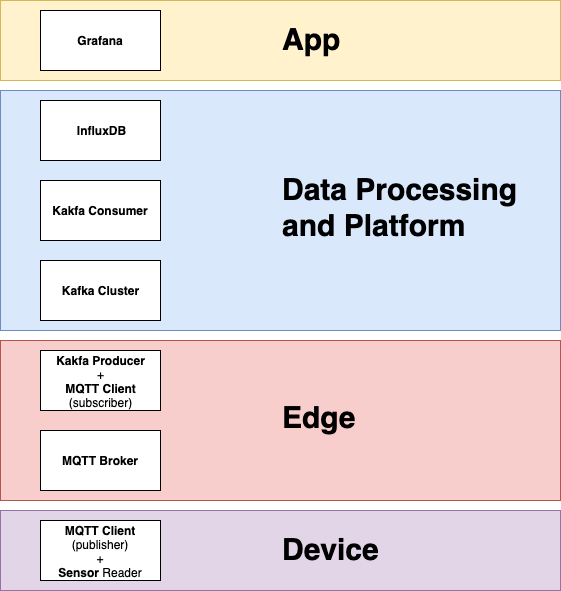
\includegraphics[height=0.8\paperheight]{design}
            \end{figure}
            
        \end{frame}

        \section{Desarrollo de solución}

        \begin{frame}
            \frametitle{Dispositivos y sensores}

            \begin{itemize}
                \item Raspberry Pi + DHT11
            \end{itemize}

            \begin{figure}[]
                \centering
                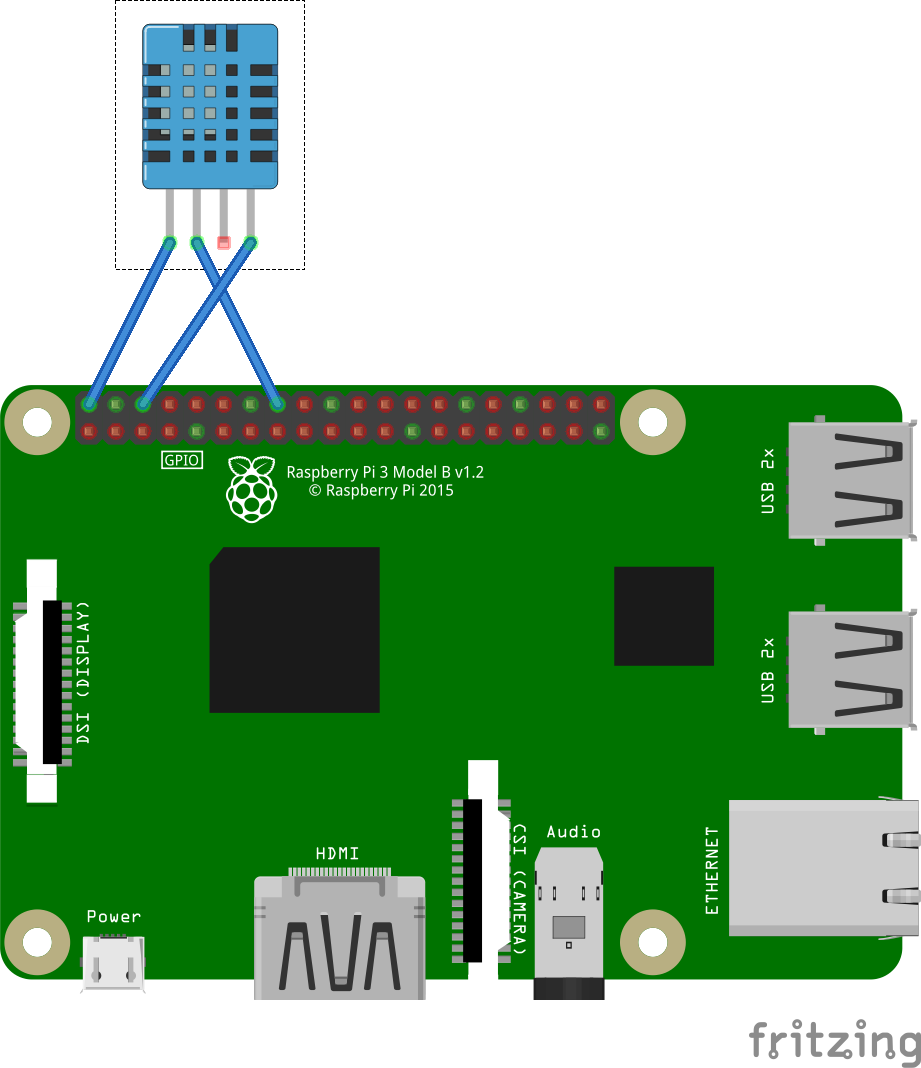
\includegraphics[height=0.6\paperheight]{schema}
            \end{figure}
        \end{frame}

        \begin{frame}
            \frametitle{Virtualización de servicios}

            \begin{itemize}
                \item Docker + Docker-compose
                \item Generar más dispositivos de los que tenemos físicamente
                \item Automatizar despliegue
                \item \textbf{Imágenes utilizadas:}
                \begin{itemize}
                    \item Eclipse Mosquitto (oficial)
                    \item bitnami/kafka
                    \item InfluxDB (oficial)
                    \item grafana/grafana
                \end{itemize}
            \end{itemize}
        \end{frame}

        \begin{frame}
            \frametitle{Desarrollo de servicios}

            \begin{itemize}
                \item Todo en Python
                \item Comportamiento básico
                \item \textbf{Librerias utilizadas:}
                \begin{itemize}
                    \item Eclipse Paho (MQTT)
                    \item Kafka-Python Client
                    \item InfluxDB-Python
                \end{itemize}
            \end{itemize}
        \end{frame}

        \begin{frame}
            \frametitle{Análisis de datos}

            \begin{itemize}
                \item Dashboard para monitorizar temperatura
                \item Temperatura actual + Evolución temporal + Temperatura media
            \end{itemize}

            \begin{figure}[]
                \centering
                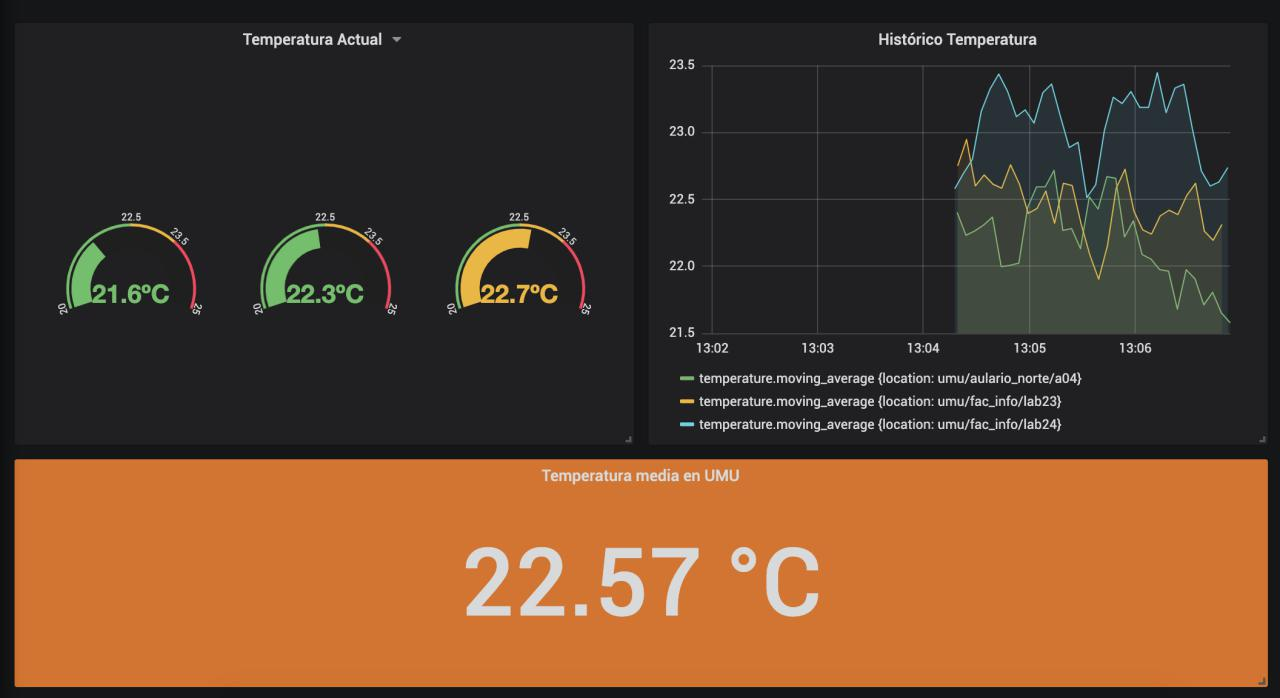
\includegraphics[height=0.5\paperheight]{dashboard}
            \end{figure}
        \end{frame}

        \section{Conclusiones}

        \begin{frame}
            \frametitle{Vías futuras}

            \begin{itemize}
                \item Profundizar en cada tecnología. Ir más allá de la prueba de concepto
                \item Análisis de idoneidad para escenarios reales
            \end{itemize}
        \end{frame}

        \begin{frame}
            \frametitle{Fin}

            \begin{center}
                \Huge \textbf{¡GRACIAS!}
            \end{center}

            \begin{itemize}
                \item Código en \url{https://github.com/adrymyry/iot-pipeline}
                \item \textbf{Ping me!}
                \begin{itemize}
                    \item @miralles en Telegram
                    \item @adrymyry everywhere :)
                    \item adrian.miralles@um.es
                \end{itemize}
            \end{itemize}
            
        \end{frame}

    \end{document}

% \title[About Beamer] %optional
% {About the Beamer class in presentation making}
 
% \subtitle{A short story}
 
% \author[Arthur, Doe] % (optional, for multiple authors)
% {A.~B.~Arthur\inst{1} \and J.~Doe\inst{2}}
 
% \institute[VFU] % (optional)
% {
%   \inst{1}%
%   Faculty of Physics\\
%   Very Famous University
%   \and
%   \inst{2}%
%   Faculty of Chemistry\\
%   Very Famous University
% }
 
% \date[VLC 2013] % (optional)
% {Very Large Conference, April 2013}
 
